\documentclass[12pt]{article}

\usepackage[spanish, es-tabla, es-nodecimaldot]{babel}
\usepackage[utf8x]{inputenc}
\usepackage{amsmath}

\usepackage{hyperref}
\usepackage{url}
\usepackage{textcomp}
\usepackage{gensymb}
\usepackage[dvipsnames]{xcolor}

\usepackage{parskip}
\usepackage{fancyhdr}
\usepackage{multicol}
\usepackage{vmargin}
\usepackage{setspace}
\usepackage{geometry}

\usepackage{float}
\usepackage{array}
\usepackage{graphicx}
\graphicspath{{images/}}
\usepackage{wrapfig}
\usepackage{caption}
\usepackage{subcaption}

\setmarginsrb{2 cm}{1 cm}{2 cm}{1.5 cm}{0.5 cm}{1 cm}{1 cm}{1 cm} %{izq}{up}{der}{down}{Encabezado}
\title{Convección}
\author{Martín Alejandro Paredes Sosa}		

\makeatletter
\let\thetitle\@title
\let\theauthor\@author
\let\thedate\@date										
\makeatother

\pagestyle{fancy}
\fancyhf{}
%\rhead{Lic.. Física}
%\lhead{Informe 5: \thetitle}
\cfoot{\thepage}

\begin{document}
%====================================================================
\begin{center}
{ \large \bfseries \thetitle}
\end{center}
	\begin{minipage}{\textwidth}
		\begin{center} 
			\theauthor 
			\end{center}
	\end{minipage}
%===================================================================================================
	\begin{abstract}
		Esta experiencia se realizaron experimento relacionados con la convección. El objetivo fue observar el fenómeno de convección natural y forzada.
	\end{abstract}
%===================================================================================================

\section{Introducción}
\vspace{-0.5cm}
La convección es una de las tres formas de transferencia de calor. Se caracteriza porque se produce por medio de un fluido (líquido o gas) que transporta el calor entre zonas con diferentes temperaturas. La convección se produce únicamente por medio de materiales, la evaporación del agua o fluidos. La convección en sí es el transporte de calor por medio del movimiento del fluido. Por ejemplo, al trasegar mediante bombas o al calentar agua en una cacerola, el agua en contacto con la base de la cacerola asciende, mientras que el agua de la superficie, desciende y ocupa el lugar que dejó la caliente.

Esta experiencia se divide en dos:

Para las dos actividades se utilizó un arreglo con una placa métalica que fue previamente calentada por contacto directo con agua a 70°C. 

En la primera actividad, la placa se colocó horizontal y verticalmente para medir la velocidad del cambio en su temperatura. A esto le llamaremos convección natural.

Para la segunda actividad, se realizó el mismo procedimiento pero esta vez colocando un generador de viento a distintas velocidades. A esto le llamaremos convección forzada.

%===================================================================================================

\section{Desarrollo Experimental}
\vspace{-0.5cm}
El desarrollo se divide en las dos actividades,:


Actividad 1 
Se calentaró la placa metálica por contacto directo con agua en cafetera y se colocó en posición horizontal para hacer el
seguimiento temporal de la temperatura. Enseguida se repitió este
procedimiento pero se colocó la placa verticalmente. En los dos
casos se tomó lecturas por 15 minutos con una frecuencia de muestreo de 30 segundos. 

Actividad 2 
El generador de viento se fijó en una posición apropiada. La placa metálica se colocó horizontalmente a una distancia de 30 cm aproximadamente.
Se realizaron mediciones de temperatura y de su variación temporal, 
Se escogió tres velocidades de viento, para cada una de las velocidades de viento se partió de aproximadamente una misma temperatura inicial de la placa. 
Se tomaron datos con una frecuencia de muestreo de 10 Hz durante 10 minutos con cada velocidad de viento.

%===================================================================================================
\pagebreak
\section{Resultados}
Los resultados también se dividen por actividad.

Para la primer actividad se construyó una gráfica del comportamiento de la temperatura en el tiempo para la placa colocada horizontalmente y la cara colocada verticalmente.

\begin{figure}[H]
\begin{center}
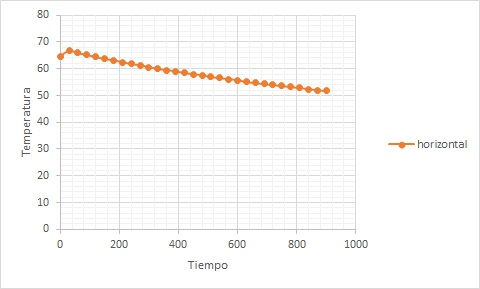
\includegraphics[width=0.7\textwidth]{horizontal1.jpg}  
\caption{Horizontal Convección Natural}
\label{uno}
\end{center}
\end{figure}

\begin{figure}[H]
\begin{center}
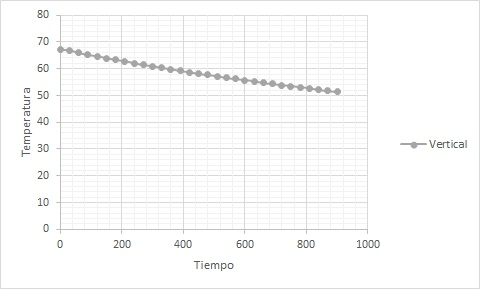
\includegraphics[width=0.7\textwidth]{vertical.jpg}  
\caption{Vertical Convección Natural}
\label{uno}
\end{center}
\end{figure}

Realizando un ajuste lineal para cada caso obtuvimos

\begin{itemize}
\item $y_h = -0.0167x +65.95$
\item $y_v = -0.0175x +66.42$
\end{itemize}

\pagebreak

Para la actividad 2 se presenta un solo gráfico de la Temperatura vs tiempo con todos los casos de las velocidades.

\begin{figure}[H]
\begin{center}
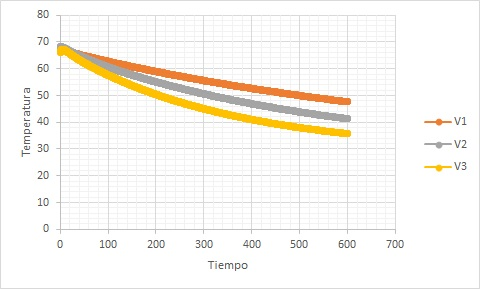
\includegraphics[width=0.7\textwidth]{34.jpg}  
\caption{Convección Forzada}
\label{uno}
\end{center}
\end{figure}

Para cuantizar las diferencias entre cada velocidad realizamos un ajuste exponencial a cada uno de los casos y obtuvimos:

\begin{itemize}
\item $y_1 = 66.303 e^{-5 \times 10^{-4} x}$
\item $y_2 = 65.661 e^{-8 \times 10^{-4} x}$
\item $y_3 = 63.511 e^{-0.001 x}$
\end{itemize}



\begin{itemize}
\item $V_1 = 1.2 m/s $
\item $V_2 = 2.6 m/s $
\item $V_3 = 6 m/s  $
\end{itemize}

%===================================================================================================



\begin{thebibliography}{6}


\bibitem{acu}
Acuña, H. (2015). \textit{Manual de Guías de Experiencias en el Laboratorio de Termodinámica Clásica}.

\bibitem{W}
Zemansky, M., Dittman, R.(1990) \textit{Calor y Termodinámica}


\end{thebibliography}
%================================================================================================


\end{document}
